\documentclass{article}

%packages
\usepackage{geometry}
\usepackage{polski}
\usepackage[utf8]{inputenc}
\usepackage{hyperref}
\usepackage{graphicx}
\graphicspath{{./assets/}}

% Margin options
\geometry{top=2.5cm}
\geometry{bottom=2.5cm}
\geometry{left=2.5cm}
\geometry{right=2.5cm}

% title
\title{Tworzenie Aplikacji na iOS}
\author{Witold Bobrowski\\Uniwersytet Jagielloński w Krakowie}
\date{Wrzesień 2018}

% Document
\begin{document}

% Title
\maketitle

%
% Section: Introduction
%
\section*{Wstęp}
W tym artykule postaram się przybliżyć proces tworzenia aplikacji
mobilnych na system operacyjny Apple iOS\@. Opowiem o najpopularniejszych 
narzędziach, wytycznych Apple, dobrych praktykach, społeczności oraz 
zaprezentuję przykładową aplikację. Aplikacja posłuży mi za punkt odniesinia 
do tych konceptów oraz paradygmatów, które tutaj przedstawię. Kod źródłowy 
zostanie udostepniony wraz z tym dokumentem, a więc zachęcam do zapoznania się 
z zawartością.


%
% Section: Environment 
%
\section*{Środowisko}

\begin{figure}[h]
\centering
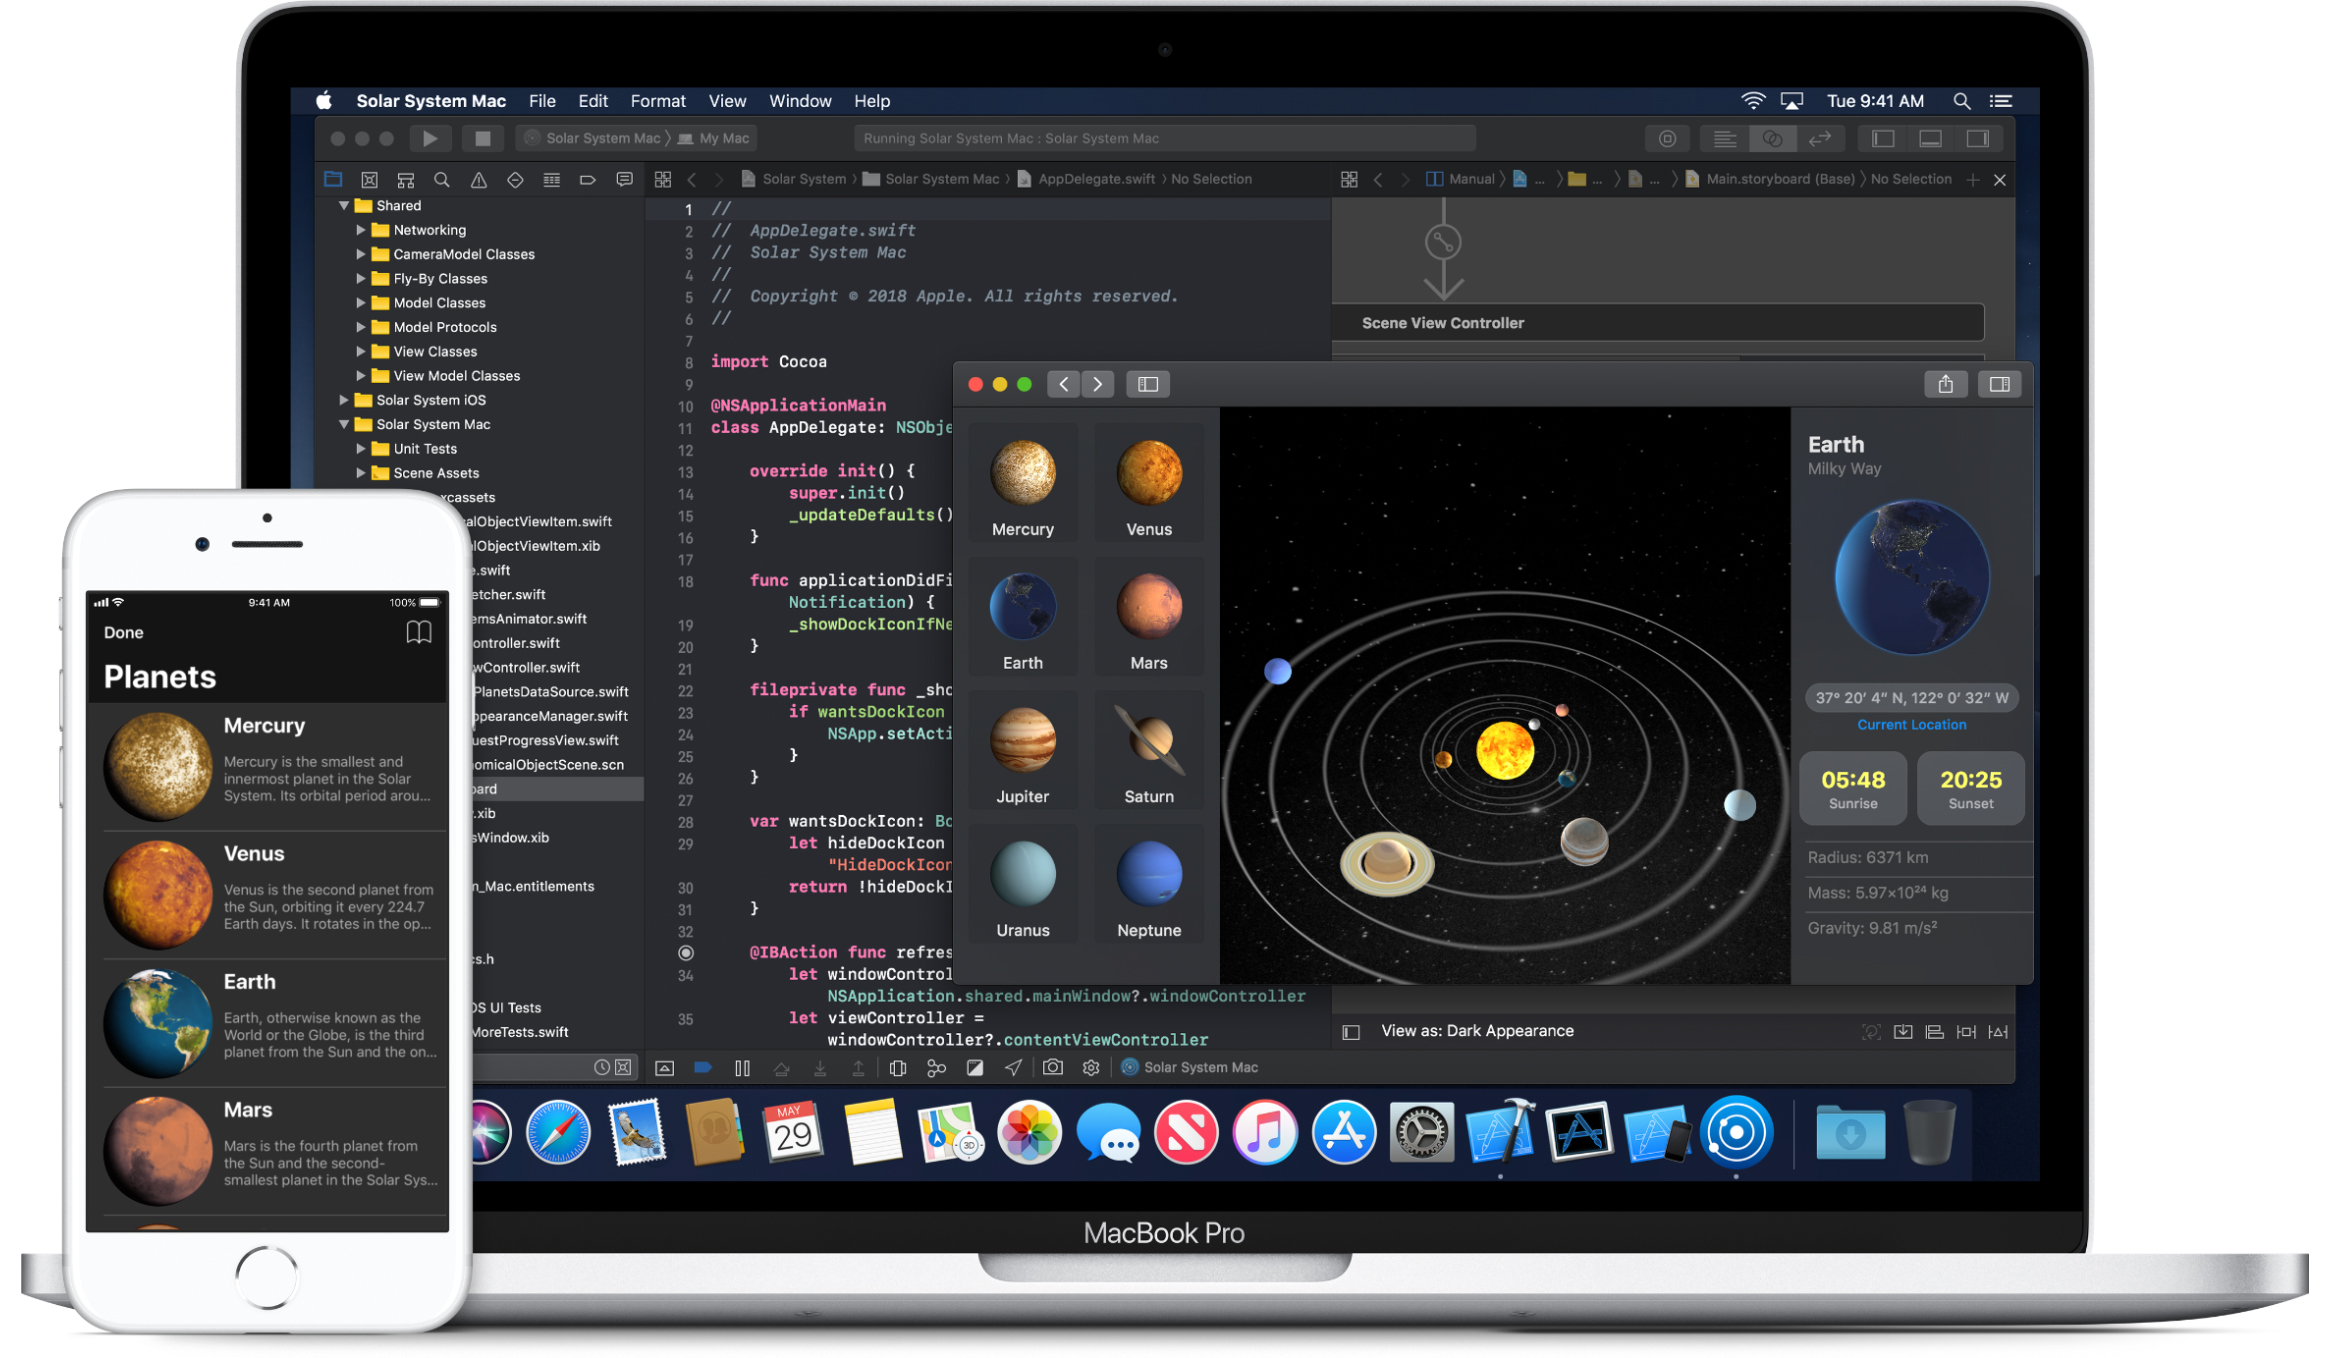
\includegraphics[width=12cm]{image-develop-hero-large_2x}
\caption{Źródło: \url{https://developer.apple.com/develop/}}
\end{figure}

\subsection*{macOS}
Na środowisko programisty tworzącego aplikaje na iOS, składa sie kilka elementów.
Przedewszystkim jest to system \textbf{macOS}, który jest dostępny jedynie na 
komputery produkowane przez Apple. Ten wymaganie powoduje, że wiele osób nie ma
nawet okazji zainteresować się tworzeniem appek na iOS bo najzwyczajniej w świecie
nie posiadają odpowiedniej maszyny. Macintosh nie cieszył się nigdy wielką
popularnością w polsce, a dla studenta może być poprostu nieosiągalny ze względu
na swoją cenę, która umiesza go w kategorii produktów premium. Technicznie jest
możliwe uruchomienie systemu na wirtualnej maszynie, bądź tak zwanym `Hackintoshu'
czyli PCecie, który dzięki zbliżonym komponentom do prawdziwego Maca pozwala przy
odrobinie wysiłku na instalację systemu macOS\@.

\subsection*{iPhone, iPad}
Naturalnie wydawało by się aby następnie wspomnieć o jakimś urządzenie z iOS, na
którym bedziemy uruchamiać aplikację. Na szczęście w naszym pakiecie narzędzi 
znajduje się symulator iOS, na którym bez problemu przetestujemy nasz kod.
Oczywiście fizyczne urządzenie pozwala nam na wiele więcej, dzięki niemu bedzięmy
mieli dostęp do wszystki funkcjonalności, których żaden symulator nie bedzie nam 
w stanie zapewnić. Więcej o symulatorze napiszę trochę później, przy okazji XCode'a.
O ile ciężko wśród znajomych znaleźć kogoś z Macintoshem, o tyle łatwiej uda nam 
się wskazać kogoś z iPhonem. Telefony Apple na dobre wkroczyły na rynek polski i 
są coraz powszechniejsze. A to z pewnością dobra wiadomość dla programistów tworzących
oprogramowanie na tą platformę. Kolejnych urządzenie może być tablet z rodziny iPad
lub najmłodszy i zapewnie ostatni potomek reliktu przeszłości: iPod Touch. Każde
z tych urządzeń różni się od siebie, lecz co najważniejsze wszystkie posiadają 
jeden system operacyjny, który na każdym z nich identycznie. Warto jednak upewnić
się, że znajdujemy się wposiadaniu takiego urządzenia, które wspiera najnowszą
wersję iOS\footnote{Podczas pisania tego artykułu najnowszą wersją jest świeżo 
upieczony iOS 12, który wspiera tak stare urządzenia jak iPhone 5S z 2012 roku}.

\subsection*{XCode}

\begin{figure}[h]
\centering
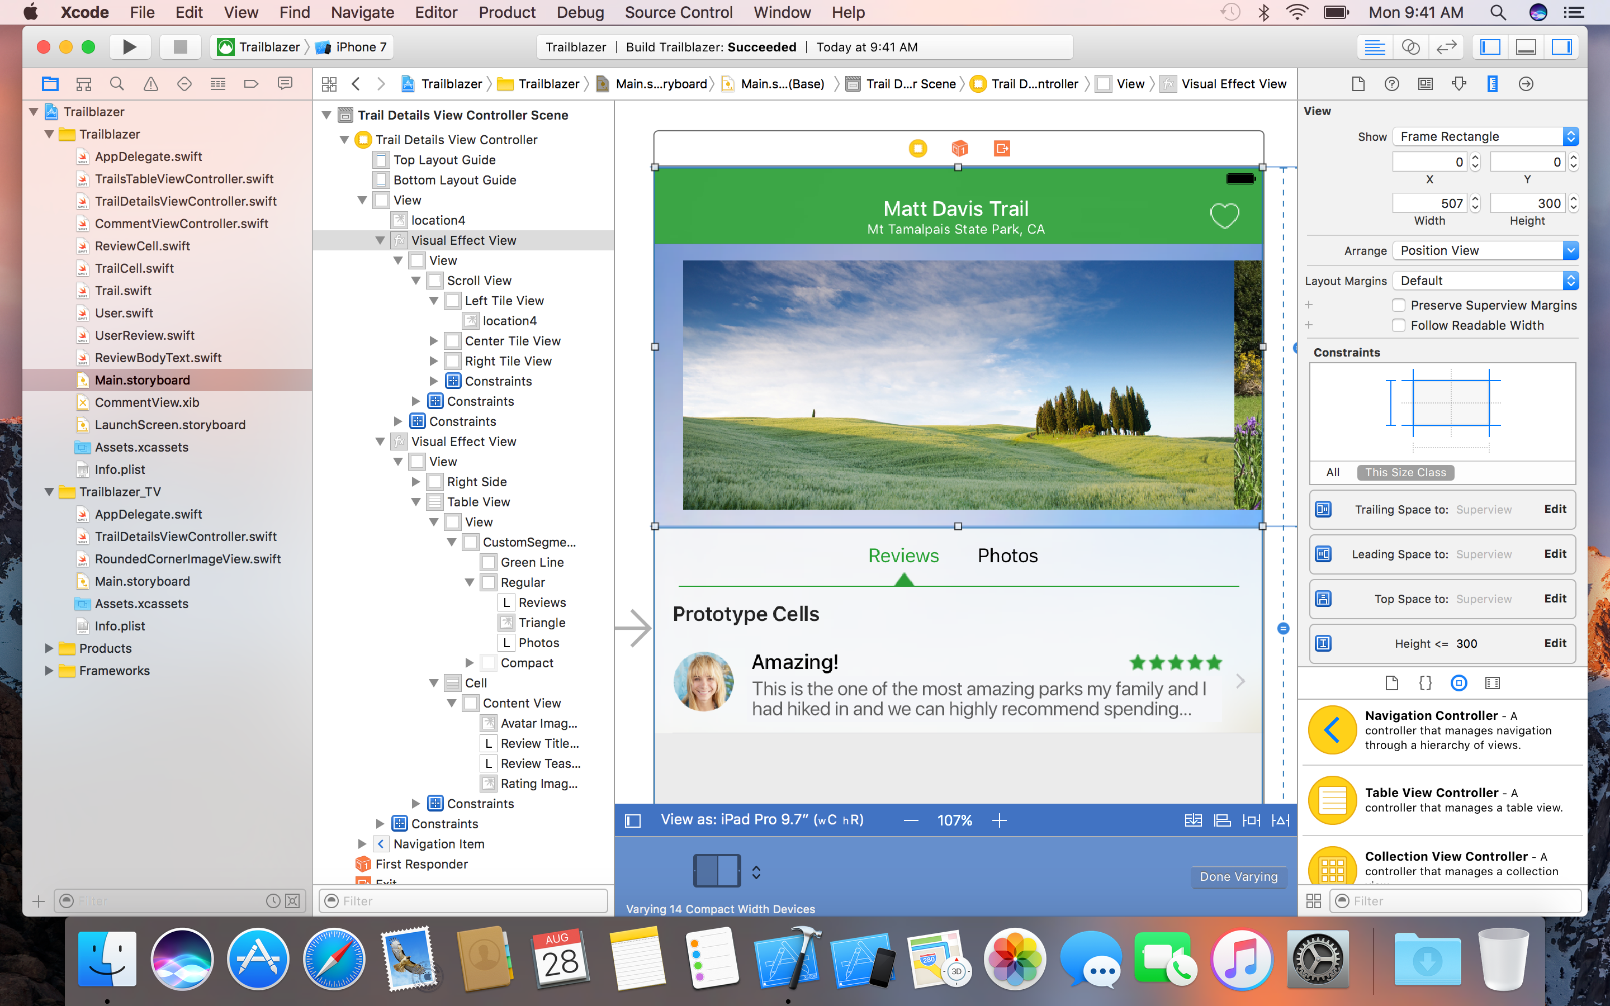
\includegraphics[width=12cm]{interface-builder_2x}
\caption{Źródło: \url{https://developer.apple.com/xcode/interface-builder/}}
\end{figure}

Wymagania hardware'owe mamy już za sobą, a więc przejdźmy do narzędzi jakimi będziemy
się posługiwać. Pierwszym z nich jest \textbf{XCode}, który przedewszystkim pełni
rolę IDE, ale również posiada zestaw dodatkowych narzędzi, między innymi wcześniej
wspomniany \textbf{Simulator} czy \textbf{Instuments}, aplikacja posiadająca mnóstwo
narzędzi analizujących wynajność aplikacji działającej na urządzeniu bądź symulatorze.
Instuments to z pewnością narzędzie, z których każdy programista iOS musi się
zapoznać, a wskazane by było skożystać z niego przed wypuszczeniem swojej aplikacji
do AppStore.

Jeżeli chodzi o Xcode jako IDE to mamy do czynienia z dość zaawansowanym programem,
który udostępnia nam takie funkcjonalności jak \textbf{Interface Builder} czy
\textbf{View Debugger}. Jest całkiem spora szansa, że już obiło się wam o uszy
jedno czy dwa słowa o XCode, i na 99\% nie było to nic pozytywnego. Niestety 
natywne IDE nie cieszy sie najlepszą reputacją, a Apple nie daje nam zbyt dużego 
wyboru uniemożliwiając tworzenia aplikacji bez chociażby minimalnej interakcji
z Xcode, który jest odpowiedzialny za zarządzanie projektem oraz co najważniejsze,
podpisywanie aplikacji certyfikatem developerskim\footnote{Aby udostępnic aplikację
w AppStore należy posiadać opłacone konto deweloperskie Apple, które kosztuje 
bagatela 99\$ rocznie.}. Istnieją alternatywy, a najpopularniejszą z nich jest
AppCode od JetBrains, lecz osobiście nie spotkałem żadnego profesjonalnego iOS
dewelopera korzystającego z tego oprogramowania. Korzystanie z AppCode nie
uwalnia nas do końca z korzystania z Xcode, co dla wielu osób wydaję się poprostu
bez celowe. Nic oczywiście nie powstrzymuje nas od edytowania plików źródłowych
w vimie, lecz wziąż będziemy musieli jakiś procent naszej pracy wykonać w Xcode.
Największą jego bolączką jest słaba stabilność, szybkość z jaką indeksuje
pliki w projekcie oraz wolne code-completion. Częścią problemu jest 
\textbf{SourceKit}, biblioteka od Apple, która odpowiedzialna jest właśnie za
indeksowanie kodu źródłowego oraz budowanie na jego podstawie drzewa (Xcode 
oddelegowuje sporo swojej pracy do SourceKitu). Aktualnie najnowszą odsłoną
Xcode jest w wersji 10.

\subsection*{Objective-C, Swift}

\begin{figure}[h]
\centering
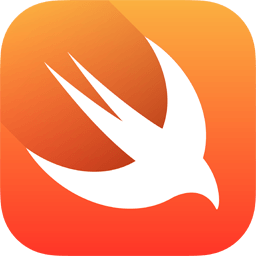
\includegraphics[width=2cm]{swift-128_2x}
\caption{Źródło: \url{https://developer.apple.com/swift/}}
\end{figure}

Objective-C było językiem w którym stworzony został framework Cocoa, pozwalający
na programowanie aplikacji na system NeXTStep, a póżniej gdy został on wykupiony 
przez apple pod koniec lat 90' XX-go wieku na platformę MacOS X. Dzięki sukcesowi
iPhone'a cieszył się on większą popularnością. I trwało to do 2014go roku gdy
został zaprezentowany język \textbf{Swift}, który zdobył serca programistów tworzących
natywny software na platformy Apple i dzisiaj już większość z nich korzysta wyłącznie
z niego.

Swift to nowoczesny język czerpiący z wielu języków najlepsze ich aspekty i 
paradygmaty. Pozwala na programowanie w pełni obiektowe, ale dzięki typom wartości
(\textit{value type semantics}) oraz przekazywanie referencji do funkcji pozwala 
również na programowanie funkcyjne. Znajdziemy w nim podobieństwa do Scali, Haskella,
Smalltalk, Clojure, Python, Ruby etc. Swift jest silnie typowanym językiem 
posiadającym klasy, których instancje przekazywane są przez referencję, struktury,
których instancje przekazywane są przez wartość, oraz protokoły, które pozwalają
na unikanie dziedziczenia poprzez stosowanie ich na klasach/strukturach. Istnieje
możliwość importowania kodu napisanego w Objective-C w Swifcie ze względu na wspólny
Runtime. Dodatkowo Swift może korzystać z kodu napisanego w C lub C++. 

Platformy, na których dostępny jest Swift to macOS, Linux oraz Windows. Jako 
projekt Open-Source jego kod źródłowy jest dostępny na portalu 
\href{https://github.com/apple/swift}{github}. W Swifcie napiszemy nie tylko
aplikację na iOS, ale również na pozostałe platformy Apple czyli macOS, watchOS
oraz tvOS\@. Isnieje również możliwość pisania serwerów, przy użyciu takich frameworków 
jak \href{https://www.kitura.io}{Kitura} czy \href{https://vapor.codes}{Vapor}.
Najnowszą wersją Swifta jest 4.2.

\subsection*{iOS SDK}
iOS dziedziczy wiele po systemie macOS\@. W skład iOS SDK (\textit{Software Development 
Kit}) wchodzą biblioteki znane już deweloperom tworzącym oprogramowanie na macOS
oraz biblioteki stworzone z myślą o urządzeniach mobilnych. CocoaTouch jest potomkiem 
frameworku Cocoa dostępnego na systemach macOS, który jest rozszerzony o interfejs 
obsługi narzędzi dostępnych w urządzeniu mobilnym takich jak rozpoznawanie gestów,
serwis lokalizacji czy obsługa kamery. W skład CocoaTouch wchodzą między innymi
biblioteki Foundation, UIKit, MapKit, EventKit i wiele innych. Dzięki temu pakietowi
Apple zdefiniowało jak powinny być tworzone aplikacje na iOS\@. Dostarczony jest 
zbiór wielu elementów interfejsu użytkownika, które można dowolnie rozszerzać i
modyfikować, aby stworzyć unikalny wygląd aplikacji trzymając się wytycznych
wyznaczonych przez Apple. Dostęp do gestów zapewni naszej aplikacji lekkość obsługi
oraz intuicyjność, a niezliczona ilość innych bibliotek wchodzących w skład
CocoaTouch sprawi, że aplikacja nabierze życia. Implementowanie funkcjonalności staje
się bardzo proste dzięki wysoko poziomowym interfejsom dającym dostęp do
poszczególnych elementów systemu oraz fizycznego urządzenia. CocoaTouch jest 
najbardziej elementarnym frameworkiem na iOS, ponieważ to on zapewnia na poziomie
podstawowym to co potrzebne do stworzenia funkcjonalnej aplikacji. 

\subsection*{AppStore}

\begin{figure}[h]
\centering
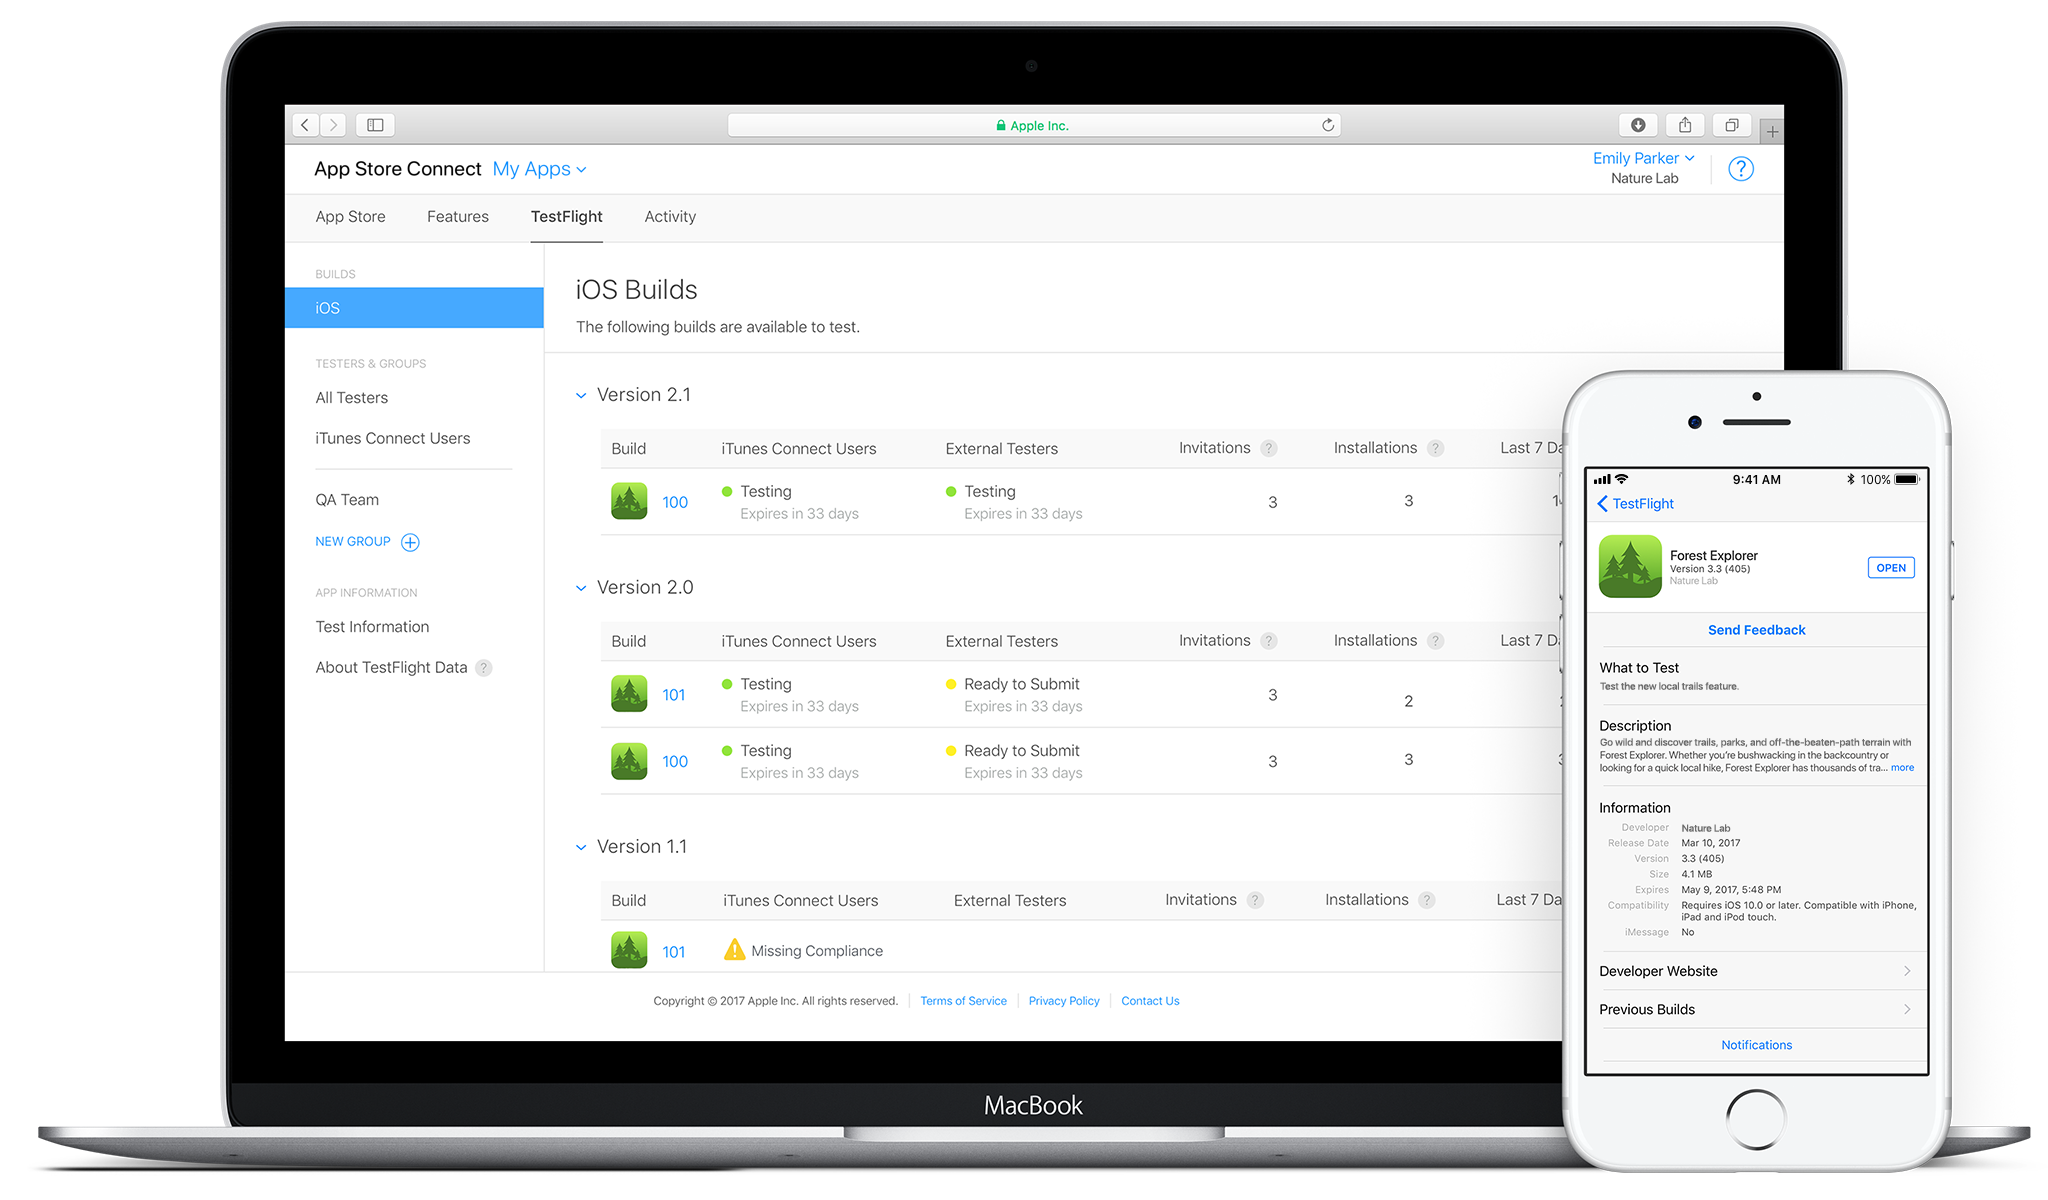
\includegraphics[width=12cm]{testflight-overview-hero-large_2x}
\caption{Źródło: \url{https://developer.apple.com/testflight/}}
\end{figure}

Jedyną oficjalną drogą udostępnienia aplikacji konsumentowi jest AppStore, świetnie
znany każdemu użytkownikowi iOS\@. Aby umieścic aplikację w sklepie AppStore
należy posiadać wcześniej wspomniane konto deweloperskie Apple. Portal AppStoreConnect
pozwoli nam na zarządzanie kolejnymi wersjami aplikacji, a nawet beta-testowanie
dzięki aplikacji TestFlight. To wszystko za jedyne 99\$ rocznie. Na iOS nie istnieje
inna możliwość instalacji aplikacji niż AppStore, za wyjątkiem manulanej instalacji
przez Xcode. W tym celu najlepiej udostępniać swój kod źródłowy na githubie. Zanim 
jednak aplikacja zostanie upubliczniona w AppStore musi ona przejsc proces Review.
Apple dokładnie analizuje każdą aplikację indywidualnie, poprzez manualne testy oraz
skrypty, które mają zapewnić bezpieczeństwo oraz upewnić się, że aplikacja spełnia
wszystkie ich wymogi odnośnie UI oraz UX\@. Proces ten może potrwać od jednego do trzech
dni, a z każdą kolejną iteracja poprawek i review okres ten będzie się przedłużał.

\end{document}
